\documentclass[10pt]{examdesign}
\usepackage{amsmath}
\usepackage{pifont}
\usepackage{graphicx}
\usepackage{multicol}

\SectionFont{\large\sffamily}
\Fullpages
\ContinuousNumbering
%\ShortKey

\DefineAnswerWrapper{}{}
\NumberOfVersions{1}

\class{{\Large Circuit Lab Test}}

\begin{document}

\begin{examtop}
    \noindent
    {\Large Circuit Lab Test - Summer Exchange (83 pts total)} \\ \\
    South Brunswick High School Science Olympiad\\
\end{examtop}


%Circuit lab
	\begin{multiplechoice}[title={Multiple Choice (2pts each, 16pts total)}, resetcounter=yes, examcolumns=2]
		\begin{question}
			When two resistors have resistances $ R_1 $ and $ R_2 $ are connected in parallel, the equivalent resistance of the combination is $ 10 \Omega $. Which of the following statements about the resistances is true? 
			\choice [!]{Both $ R_1 $ and $ R_2 $ are greater than $ 10 \Omega $.}
			\choice {Both $ R_1 $ and $ R_2 $ are equal to $ 10 \Omega $.}
			\choice {Both $ R_1 $ and $ R_2 $ are less than $ 10 \Omega $.}
			\choice {The sum of $ R_1 $ and $ R_2 $ is $ 10 \Omega $.} 
			\choice {One of the resistances is greater than $ 10 \Omega $, and the other is less than $ 10 \Omega $.}
		\end{question}
		\begin{question}
			When two identical resistors are connected in series to a battery, the total power dissipated is $ P $. When the same two resistors are connected in parallel to the same battery, the total power dissipated is 
			\choice {$ \dfrac{1}{4} P $}
			\choice {$ \dfrac{1}{2} P $}
			\choice {$ P $}
			\choice {$ 2P $}
			\choice [!]{$ 4P $}
		\end{question}
		\begin{question}
			A magnetic field perpendicular to the plane of a wire loop is uniform in space but changes with time $ t $ in the region of the loop. If the induced emf in the loop increases linearly with time $ t $, then the magnitude of the magnetic field must be proportional to 
			\choice {$ t^3 $}
			\choice [!]{$ t^2 $}
			\choice {$ t $}
			\choice {$ t^0 $}
			\choice {$ t^{1/2} $}
		\end{question}
		\begin{question}
			Which of the following combinations of values for total resistance, $ R $, and capacitance, $ C $, would produce an $ RC $ circuit that reached its maximum charge (on the capacitor) most quickly?
			\choice [!]{$ R = 4 \Omega $; $ C = 20 \mu F $}
			\choice {$ R = 6 \Omega $; $ C = 35 \mu F $}
			\choice {$ R = 8 \Omega $; $ C = 30 \mu F $}
			\choice {$ R = 4 \Omega $; $ C = 35 \mu F $}
			\choice {$ R = 8 \Omega $; $ C = 40 \mu F $}
		\end{question}
		\begin{question}
			A battery whose emf is $ 40 V $ has an internal resistance of $ 5 \Omega $. If the battery is connected to a $ 15 \Omega $ resistor $ R $ , what will the voltage drop across $ R $ be?
			\choice {10V}
			\choice [!]{30V}
			\choice {40V}
			\choice {50V}
			\choice {70V}
		\end{question}
		\begin{question}
			A given circuit uses 125 watts of power. If the circuit has a total resistance of $ 5 \Omega $, at what voltage must it be operating
			\choice {5V}
			\choice {15V}
			\choice [!]{25V}
			\choice {45V}
			\choice {625V}
		\end{question}
		\begin{question}
			The slope of a charge vs. time graph for an $ RC $ circuit represents 
			\choice {the total charge on the capacitor plates}
			\choice {the potential energy of the capacitor}
			\choice {the resistance of the circuit}
			\choice {the instantaneous voltage of the capacitor}
			\choice [!]{the instantaneous current of the circuit}
		\end{question}
		\begin{question}
			How many windings must a solenoid of length $ 80 cm$ have in order to establish a magnetic field of strength $ 0.2 T $ inside the solenoid, if it carries a current of $ 20A $
			\choice {1000}
			\choice [!]{6400}
			\choice {10000}
			\choice {32000}
			\choice {64000}
		\end{question}
	\end{multiplechoice}

    \begin{shortanswer}[title={Short Answer, 52 pts total},rearrange=no,resetcounter=no]
        \begin{question}
        Provide formulas for the following: (4pts)
        \\a. Work (W) as a function of Voltage (V), Current (I), and Time (T)
        \\b. Energy (E) as a function of Voltage (V), Resistance (R), and Time (T)
        \\c. Charge (Q) as a function of Current (I) and Time (T)
        \\d. Current (I) as a function of Power (P) and Resistance (R)
        
        \begin{answer}
        W=VIT
        $E=V^2 T/R$
        Q=IT
        I=$\sqrt{\frac{P}{R}}$
        \end{answer}
        \end{question}
        \begin{question}
        What SI unit is $V^2F$ equal to? (V stands for Volts and F for Farad)? (2pts)
        \begin{answer}
        Joule (J)
        \end{answer}
        \end{question}
        \begin{question}
        What is Kirchoff's Voltage Law? (2pts)
        \begin{answer}
        for a closed loop series path the algebraic sum of all the voltages around any closed loop in a circuit is equal to zero
        \end{answer}
        \end{question}
        \begin{question}
        What is Kirchoff's Current Law? (2pts)
        \begin{answer}
        At any node (junction) in an electrical circuit, the sum of currents flowing into that node is equal to the sum of currents flowing out of that node
        \end{answer}
        \end{question}
        \begin{question}
        How does an inductor work? Explain the theory and concepts behind an inductor. (4 pts)
        \begin{answer}
        \end{answer}
        \end{question}
        \begin{question}
        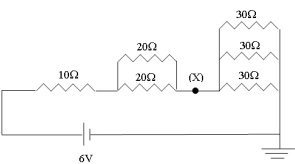
\includegraphics[width=5cm]{circuit1.png}
        \\For the circuit above, answer the following. (6pts)
        \\a. Calculate the value of the voltage at point (X). 
        \\b. What is the total current out of the 6V battery? 
        \\c. What is total work/energy out of the circuit after an hour? 
        \begin{answer}
        a. 2 V
        b. 0.2 A
        c. 43.2 kW
        \end{answer}
        \end{question}
        \begin{question}
        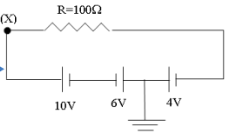
\includegraphics[width=5cm]{circuit2.png}
        \\For the circuit above, answer the following: (6pts)
        \\a. What is the value of the potential (voltage) at point (X)?
        \\b. What is the current across the 100Ω resistor? 
        \\c. What is the power across the 100Ω resistor?
        \begin{answer}
        a. 4 V
        b. 0.08 A
        c. 0.64 W
        \end{answer}
        \end{question}
        \begin{question}
        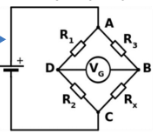
\includegraphics[width=5cm]{circuit3.png}
        \\For the Wheatstone Bridge above, we are searching for an unknown Rx given known values for $R_1$, $R_2$, and $R_3$. (4pts)
        \\a. If R1 = 57 kΩ, R2= 2.2MΩ, and R3= 1Ω, what must Rx equal to make this Wheatstone Bridge circuit “balanced”?
        \begin{answer}
        38.6 Ohms
        \end{answer}
        \end{question}
        \begin{question}
        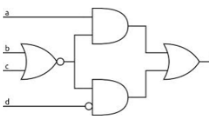
\includegraphics[width=5cm]{circuit4.png}
        \\Please convert the logic gate circuit into boolean expressions (ex. AB+C,DC,etc.) Answer for the output in terms of A, B, C, D. You do not need to simplify. (4pts)
        
        \begin{answer}
        a. A $\overline{b}\overline{c}+\overline{b}+\overline{c}+\overline{d}$
        \end{answer}
        \end{question}
        \begin{question}
        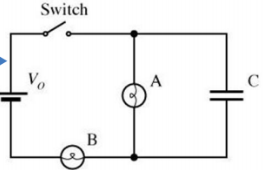
\includegraphics[width=5cm]{circuit5.png}
        \\Please solve for the following with the circuit to the right, assuming that the switch is closed for a very long time, until t=0 and then the switch is opened for a very long time. Vo=12V, each light bulb has 3Ω resistance and the Capacitor is 200mF. (6pts)
        \\a. What is the voltage across the Capacitor at t=0
        \\b. What is the time constant of the circuit when t is greater than 0 (2 points)
        \\c. What is the complete formula for the voltage of the capacitor for all time, when t is greater than 0 (3 points)
        \begin{answer}
        a. 6 V
        b. 0.6 sec
        c. $6 V\times e^\frac{-t}{0.6 sec}$
        \end{answer}
        \end{question}
        \begin{question}
        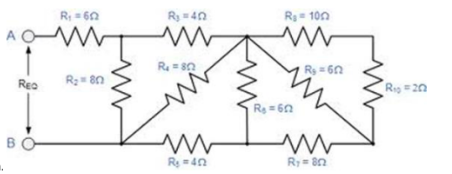
\includegraphics[width=10cm]{circuit6.png}
        \\Solve for the equivalent resistance between nodes a and b. (4pts)
        \begin{answer}
        10 Ohms
        \end{answer}
        \end{question}
        \begin{question}
        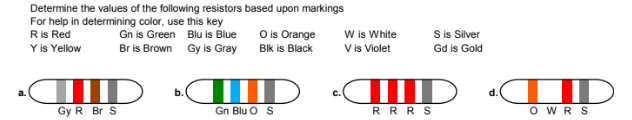
\includegraphics[width=15cm]{circuit7.png}
        \\Determine the values and tolerance of each of the following resistors based upon markings, read from left to right. (8pts, 1pt for resistance, 1pt for tolerance)
        \begin{answer}
        a. 820 Ohms, 10 percent
        b. 56,000 Ohms, 10 percent
        c. 2,200 Ohms, 10 percent
        d. 3,900 Ohms, 10 percent
        \end{answer}
        \end{question}
    \end{shortanswer}
	\pagebreak
	\begin{shortanswer}[title={Free Response (15 pts)},rearrange=no,resetcounter=no]
		\begin{question}
				The diagram below shows an uncharged capacitor, two resistors, and a battery whose emf is $ \mathcal{E} $ \\
				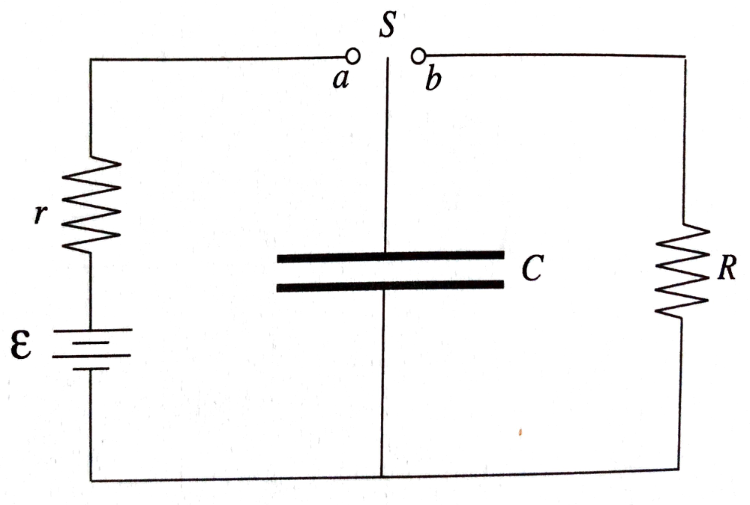
\includegraphics[width=10cm]{c1}
				\\
				The switch $ S $ is turned to a point $ a $ at time $ t = 0 $ 
				(Express all answers in terms of $ C $, $ r $, $ R $, $ \mathcal{E} $, and fundamental constants)
				\begin{enumerate}
					\item Determine the current through $ r $ at time $ t = 0 $ (2pts)
					\item Compute the time required for the charge on the capacitor to reach one-half its final value? (2pts)
					\item When the capacitor is fully charged, which plate is positively charged? (2pts)
					\item Determine the electrical potential energy stored in the capacitory when the current through r is zero (2pts)
				\end{enumerate}
				When the current through $ r $ is zero, the switch $ S $ is moved to Point $ b $; for the following parts, consider this event time $ t = 0 $
				\begin{enumerate}
					\item Determine the current through $ R $ as a function of time. (2pts)
					\item Find the power dissipated in $ R $ as a function of time (2 pts)
					\item Determine the total amount of energy dissipated as hear by $ R $ (3pts).
				\end{enumerate}
			\begin{answer}
				ANSWER
				\begin{enumerate}
					\item $ I_0 = \mathcal{E}/r $
					\item $ t = (\ln 2)rC $
					\item Top plate will be positively charged
					\item $ U_E = \dfrac{1}{2} CV^2 = \dfrac{1}{2}C \mathcal{E} ^2$
				\end{enumerate}
				Second Part
				\begin{enumerate}
					\item $ I(t) = (\mathcal{E}/R)e^{-t/RC} $
					\item $ P(t) = \dfrac{\mathcal{E}^2}{R} e^{-2t/RC}$
					\item $ E = \dfrac{C \mathcal{E}^2}{2} $
				\end{enumerate}
			\end{answer}
		\end{question}
	\end{shortanswer}
\end{document}